\chapter{Estimation of Required Number of Samples}

\section{Brute Force Estimation}

First an estimate for the number of samples needed to achieve different confidence level and intervals is investigated. The number of samples needed is found using the normal approximation of the Binomial proportion \citep{SampleNumURC}. 

\begin{equation}\label{eq:numSamples}
\frac{z_{\frac{\alpha}{2}} \sqrt{\frac{\hat{\gamma}\left(1-\hat{\gamma}\right)}{N}}}{\hat{\gamma}} < m
\end{equation} 
\begin{where}
\va{$z_{\frac{\alpha}{2}}$}{is the $100(1-\frac{\alpha}{2})$-th percentile of the standard normal distribution}{1}
\va{$\hat{\gamma}$}{is the estimated probability}{1}
\va{N}{is the number of samples}{1}
\va{m}{is the margin around $\hat{\gamma}$}{1}
\end{where}

From the \autoref{chap:introduction} the value of $\hat{\gamma}$ is set to $10^{-5}$. With that estimations of the number of samples needed to uphold different confidence level and intervals can be found as seen in \autoref{tab:numSample}. 

\begin{table}[H]
\centering
\begin{tabular}{c|l|l|l|l|l|l|}
\multicolumn{2}{l}{}  & \multicolumn{5}{c}{\textbf{Confidence level}} \\ \cline{3-7} 
\multicolumn{2}{l|}{}  & \textbf{80 \%} & \textbf{85 \%} & \textbf{90 \%} & \textbf{95 \%} & \textbf{99 \%} \\ \cline{2-7} 
\multirow{5}{*}{{\rotatebox{90}{\textbf{Confidence interval}}}} & \textbf{$\pm$0.5 dB} & 11.0E+6 & 13.9E+6 & 18.2E+6 & 25.8E+6 & 44.6E+6 \\ \cline{2-7} 
 & \textbf{$\pm$1 dB} 	& 2.45E+6 	& 3.09E+6 	& 4.04E+6 	& 5.73E+6 	& 9.90E+6 \\ \cline{2-7} 
 & \textbf{$\pm$1.5 dB} & 965E+3 	& 1.22E+6 	& 1.59E+6 	& 2.26E+6 	& 3.90E+6 \\ \cline{2-7} 
 & \textbf{$\pm$2 dB} 	& 480E+3 	& 606E+3 	& 791E+3 	& 1.12E+6 	& 1.94E+6 \\ \cline{2-7} 
 & \textbf{$\pm$2.5 dB} & 271E+3 	& 342E+3 	& 447E+3 	& 634E+3 	& 1.10E+6 \\ \cline{2-7} 
\end{tabular}
\caption{Estimated number of samples for different confidence levels and intervals.}
\label{tab:numSample}
\end{table}

\newpage
\subsection{Statistics method for rare events}
As seen in \autoref{tab:numSample}, there is a need of a high number of samples, to get a high confidence interval. The reason for this, is the need for a high number of rare events to occur to get a high confidence interval for these events. 

For simulation purposes there have been developed some methods to handle this problem. One of them is importance sampling. Importance sampling changes the distribution where the samples is taken from. By changing the distribution, so the rare events is not rare anymore and a high number of them can be samples with a smaller sample population. When introducing this new distribution, there is also introduced a weighting factor. This weighting factor is defined from the change in the distribution. This weighting factor is used to go from the actual distribution to the desired distribution. However this can not be used as the measurements are taken physically with no a priori knowledge of the behaviour of the environment. Another way to look at this is to see the change in distribution as force fully introducing more spots with deep fades, that might be possible but without full knowledge of the changes it will only skew the results.

Most of the other methods \todo{what other methods} used in simulation to handle this problem with rare events, also changes the distribution, as this is one of the known parameters for simulations and can therefore not be used. 


As no useful statistical method has been found the required number of samples can not be reduced from \autoref{tab:numSample}. Therefore a compromise between the necessary number of samples, the more samples needed the longer it will take, and the confidence level and interval needs to be found. It is chosen to go for a 90\% confidence level and a 1 dB margin, as this is found to be a reasonable compromise. This means that $4.04E+6$ samples should be obtained during the measurement campaign. 

%Reduction of number of samples
%- Important sampling
%- Not useful

\section{Bootstrap Percentile Method}
Another statistically aspect, for which there are different method and techniques, is how to determine the confidence interval at a certain confidence level from the measurements. From the previous section the number of samples needed to attain a confidence level of 90\% and a margin of 1 dB is found. However this is estimated based on theory and has no particular onset in the actual measurements, it is therefore necessary to find a method to evaluate the confidence based on the measurements. The method chosen is the \textit{Bootstrap Percentile Method} \citep{Bootstrap}.

The Bootstrap method works on a surrogate population, a subset from the total sample space, which is considered an estimate of the true sample population \citep{Bootstrap}. This surrogate population will consists of the samples from the measurements campaign. For the sake of further explanations lets call the surrogate population $\mathbf{X}$ consisting of $(X_1, X_2,..X_n)$ and the value that wish to find the confidence around $\hat{\gamma}$. A new subset is now found from the surrogate population, this is done by copying randomly a value from $\mathbf{X}$ and putting it into the new subset $\mathbf{X_B}$ until $\mathbf{X_B}$ has the same size as $\mathbf{X}$. The value of $\hat{\gamma_B}$ is then found and the process is repeated a couple thousand times. All the new values of $\hat{\gamma_B}$ can then be sorted and the the desired percentile can be picked so that the lowest and highest values is left out. This will produce a the confidence interval given a confidence level \citep{Bootstrap}. For the measurements the 90 \% confidence level is picked leaving out the top and bottom 5 \% of the sorted values.

This method is only valid if the assumption of a symmetric distribution around $\hat{\gamma}$ holds \citep{Bootstrap}, which means that a high number of samples is still needed to obtain a sufficient resolution of the CDF. 

An example have been simulated in matlab, where there have been taken $4.04 \cdot 10^6$ sample from $raylrnd$. These values are converted to dB, which give a CDF, which is the yellow line in \autoref{BS90}. By using the booth strap method 10.000 times and make a CDF for each trial. By taking the 500th highest and lowest value in each point in the CDF (which gives a 90\% confidence level), a interval is created, which is shown in \autoref{BS90}. It is seen that at low procentence level, that the interval becomes wider, as there is a less sample population for that part. At the $10^{-5}$ point, there is a interval on 1.63 dB, which lower than the wanted confidence interval for this number of samples. 

\begin{figure}[H]
\center
% This file was created by matlab2tikz.
%
%The latest updates can be retrieved from
%  http://www.mathworks.com/matlabcentral/fileexchange/22022-matlab2tikz-matlab2tikz
%where you can also make suggestions and rate matlab2tikz.
%
\definecolor{mycolor1}{rgb}{0.00000,0.44700,0.74100}%
\definecolor{mycolor2}{rgb}{0.85000,0.32500,0.09800}%
\definecolor{mycolor3}{rgb}{0.92900,0.69400,0.12500}%
%
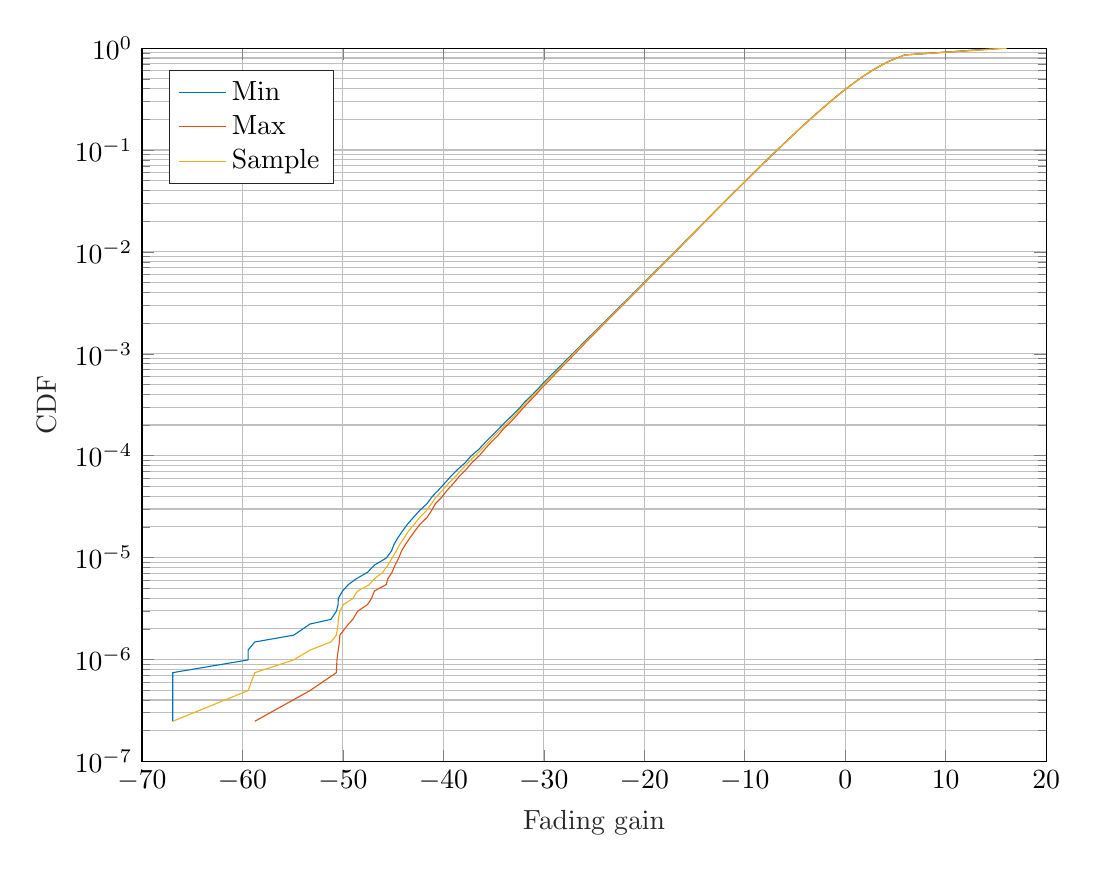
\begin{tikzpicture}

\begin{axis}[%
width=4.521in,
height=3.566in,
at={(0.758in,0.481in)},
scale only axis,
xmin=-70,
xmax=20,
xlabel style={font=\color{white!15!black}},
xlabel={Fading gain},
ymode=log,
ymin=1e-07,
ymax=1,
yminorticks=true,
ylabel style={font=\color{white!15!black}},
ylabel={CDF},
axis background/.style={fill=white},
xmajorgrids,
ymajorgrids,
yminorgrids,
legend style={at={(0.03,0.97)}, anchor=north west, legend cell align=left, align=left, draw=white!15!black}
]
\addplot [color=mycolor1]
  table[row sep=crcr]{%
-66.9341548867478	2.47524752475248e-07\\
-66.9341548867478	2.47524752475248e-07\\
-66.9341548867478	2.47524752475248e-07\\
-66.9341548867478	4.95049504950495e-07\\
-66.9341548867478	4.95049504950495e-07\\
-66.9341548867478	4.95049504950495e-07\\
-66.9341548867478	7.42574257425743e-07\\
-66.9341548867478	7.42574257425743e-07\\
-66.9341548867478	7.42574257425743e-07\\
-59.4401305500329	9.9009900990099e-07\\
-59.4401305500329	1.23762376237624e-06\\
-59.4401305500329	1.23762376237624e-06\\
-58.7667416700321	1.48514851485149e-06\\
-54.8930241094094	1.73267326732673e-06\\
-53.273131300811	2.22772277227723e-06\\
-51.1950865851036	2.47524752475248e-06\\
-50.6510586185259	2.97029702970297e-06\\
-50.4744372709179	3.46534653465347e-06\\
-50.4637174371534	3.96039603960396e-06\\
-50.0349816474052	4.7029702970297e-06\\
-49.447561740496	5.44554455445545e-06\\
-48.6769735680418	6.18811881188119e-06\\
-47.5399711931716	7.17821782178218e-06\\
-46.8753928436756	8.41584158415842e-06\\
-45.6763991666034	9.9009900990099e-06\\
-45.1564337798158	1.16336633663366e-05\\
-44.9298596668173	1.33663366336634e-05\\
-44.5379088207656	1.55940594059406e-05\\
-44.0575718584017	1.83168316831683e-05\\
-43.5660734665178	2.12871287128713e-05\\
-42.9948512600283	2.47524752475248e-05\\
-42.3622899660794	2.8960396039604e-05\\
-41.6199358073098	3.39108910891089e-05\\
-41.1423370522164	3.93564356435644e-05\\
-40.4841078412275	4.6039603960396e-05\\
-39.857584354168	5.37128712871287e-05\\
-39.2670584920207	6.26237623762376e-05\\
-38.6186456508553	7.27722772277228e-05\\
-37.8483352480315	8.49009900990099e-05\\
-37.2615291501811	9.9009900990099e-05\\
-36.4664435081505	0.000115594059405941\\
-35.8398307450146	0.000134653465346535\\
-35.1739394623042	0.000157178217821782\\
-34.4958619719187	0.000183168316831683\\
-33.8453421253092	0.000213613861386139\\
-33.1379005529252	0.000249257425742574\\
-32.4534272867472	0.000290594059405941\\
-31.8719464595624	0.000338861386138614\\
-31.1600866974086	0.000395049504950495\\
-30.5104116487686	0.000460643564356436\\
-29.8875733833693	0.000537128712871287\\
-29.1925230159786	0.000626485148514851\\
-28.509464204124	0.000730445544554455\\
-27.857506994666	0.000851980198019802\\
-27.1579158890096	0.000993316831683168\\
-26.4963734209069	0.00115841584158416\\
-25.84819948	0.00135074257425743\\
-25.1417352961274	0.001575\\
-24.4685155509094	0.00183663366336634\\
-23.7925623115133	0.00214158415841584\\
-23.1046732907459	0.00249727722772277\\
-22.4245115748514	0.00291212871287129\\
-21.7319846270678	0.00339579207920792\\
-21.0413961200324	0.00395990099009901\\
-20.3700734106301	0.00461757425742574\\
-19.7165909360272	0.00538440594059406\\
-19.048254838966	0.00627871287128713\\
-18.3494588522984	0.00732153465346535\\
-17.6687597045041	0.00853762376237624\\
-16.9973664149735	0.00995569306930693\\
-16.3241845032136	0.0116091584158416\\
-15.6565228007745	0.0135371287128713\\
-14.9778563762632	0.0157856435643564\\
-14.3116483373593	0.0184074257425743\\
-13.6354168211405	0.021464603960396\\
-12.9694492193535	0.0250294554455446\\
-12.2899458156387	0.0291866336633663\\
-11.6173489087002	0.0340341584158416\\
-10.9386885879022	0.0396868811881188\\
-10.2547448339354	0.0462782178217822\\
-9.56810854700078	0.053964603960396\\
-8.88412988229469	0.0629274752475247\\
-8.19296036845975	0.0733789603960396\\
-7.49428466079557	0.0855660891089109\\
-6.79293599216312	0.0997777227722772\\
-6.07911816926394	0.116349504950495\\
-5.36486904412886	0.135673514851485\\
-4.64011090415592	0.158207178217822\\
-3.90477194894915	0.184483663366337\\
-3.15635067132357	0.21512400990099\\
-2.38976786317853	0.250853217821782\\
-1.60200266849145	0.292516831683168\\
-0.790447628920999	0.341100247524752\\
0.0577709840127455	0.397752722772277\\
0.952604973467778	0.463814603960396\\
1.9191192375189	0.540848267326733\\
2.99103300332483	0.630676485148515\\
4.24607403431766	0.73542400990099\\
5.90663827771986	0.857568564356436\\
15.5693242968268	1\\
};
\addlegendentry{Min}

\addplot [color=mycolor2]
  table[row sep=crcr]{%
-58.7667416700321	2.47524752475248e-07\\
-58.7667416700321	2.47524752475248e-07\\
-58.7667416700321	2.47524752475248e-07\\
-53.273131300811	4.95049504950495e-07\\
-53.273131300811	4.95049504950495e-07\\
-53.273131300811	4.95049504950495e-07\\
-50.6510586185259	7.42574257425743e-07\\
-50.6510586185259	7.42574257425743e-07\\
-50.6510586185259	7.42574257425743e-07\\
-50.5919390061905	9.9009900990099e-07\\
-50.4637174371534	1.23762376237624e-06\\
-50.4637174371534	1.23762376237624e-06\\
-50.3440706249169	1.48514851485149e-06\\
-50.3046469331683	1.73267326732673e-06\\
-49.447561740496	2.22772277227723e-06\\
-49.0161929186305	2.47524752475248e-06\\
-48.535105408426	2.97029702970297e-06\\
-47.5399711931716	3.46534653465347e-06\\
-47.1639493664595	3.96039603960396e-06\\
-46.8575795211044	4.7029702970297e-06\\
-45.6763991666034	5.44554455445545e-06\\
-45.5307982428824	6.18811881188119e-06\\
-45.1081260928216	7.17821782178218e-06\\
-44.8102255669309	8.41584158415842e-06\\
-44.4474563610161	9.9009900990099e-06\\
-44.1579922321984	1.16336633663366e-05\\
-43.7871202730464	1.33663366336634e-05\\
-43.3399306777682	1.55940594059406e-05\\
-42.8191176994603	1.83168316831683e-05\\
-42.3134191700008	2.12871287128713e-05\\
-41.6220147107292	2.47524752475248e-05\\
-41.1782436924644	2.8960396039604e-05\\
-40.7851999943895	3.39108910891089e-05\\
-40.1352217887806	3.93564356435644e-05\\
-39.6065852083882	4.6039603960396e-05\\
-38.9739050365626	5.37128712871287e-05\\
-38.4219740956598	6.26237623762376e-05\\
-37.7647306261191	7.27722772277228e-05\\
-37.1809570105187	8.49009900990099e-05\\
-36.4661402484622	9.9009900990099e-05\\
-35.8816411937565	0.000115594059405941\\
-35.2712829726549	0.000134653465346535\\
-34.5863879645749	0.000157178217821782\\
-34.0201869380857	0.000183168316831683\\
-33.3082153989258	0.000213613861386139\\
-32.6927475509764	0.000249257425742574\\
-32.108399062119	0.000290594059405941\\
-31.4697382045003	0.000338861386138614\\
-30.8077506469015	0.000395049504950495\\
-30.2232624947856	0.000460643564356436\\
-29.5524959991952	0.000537128712871287\\
-28.9215341080246	0.000626485148514851\\
-28.2672640557339	0.000730445544554455\\
-27.589769514021	0.000851980198019802\\
-26.9512641716128	0.000993316831683168\\
-26.2948391782956	0.00115841584158416\\
-25.6474627887966	0.00135074257425743\\
-24.9752542562569	0.001575\\
-24.3057361435263	0.00183663366336634\\
-23.639019374287	0.00214158415841584\\
-22.9639839564226	0.00249727722772277\\
-22.2876996599225	0.00291212871287129\\
-21.6118999208888	0.00339579207920792\\
-20.924328107813	0.00395990099009901\\
-20.2626669653765	0.00461757425742574\\
-19.620759632621	0.00538440594059406\\
-18.9595810812098	0.00627871287128713\\
-18.2674289484002	0.00732153465346535\\
-17.5905419892636	0.00853762376237624\\
-16.9276365468286	0.00995569306930693\\
-16.2585942053762	0.0116091584158416\\
-15.5963726868015	0.0135371287128713\\
-14.9223906346817	0.0157856435643564\\
-14.2585851076399	0.0184074257425743\\
-13.5863909332725	0.021464603960396\\
-12.925550759673	0.0250294554455446\\
-12.2479928465401	0.0291866336633663\\
-11.5783933201661	0.0340341584158416\\
-10.9027410605745	0.0396868811881188\\
-10.2215347879431	0.0462782178217822\\
-9.53808581344148	0.053964603960396\\
-8.85624994980896	0.0629274752475247\\
-8.1668048937213	0.0733789603960396\\
-7.46952828099327	0.0855660891089109\\
-6.77027758467698	0.0997777227722772\\
-6.05783088036019	0.116349504950495\\
-5.34533305827847	0.135673514851485\\
-4.62191594844783	0.158207178217822\\
-3.88757629130586	0.184483663366337\\
-3.14066720125187	0.21512400990099\\
-2.37553244398078	0.250853217821782\\
-1.58855186388765	0.292516831683168\\
-0.777374980868274	0.341100247524752\\
0.0691904544800965	0.397752722772277\\
0.963203456043074	0.463814603960396\\
1.92927984421496	0.540848267326733\\
3.00047927642411	0.630676485148515\\
4.25518271674558	0.73542400990099\\
5.91548815268154	0.857568564356436\\
16.0736778133749	1\\
};
\addlegendentry{Max}

\addplot [color=mycolor3]
  table[row sep=crcr]{%
-66.9341548867478	2.47524752475248e-07\\
-66.9341548867478	2.47524752475248e-07\\
-66.9341548867478	2.47524752475248e-07\\
-59.4401305500329	4.95049504950495e-07\\
-59.4401305500329	4.95049504950495e-07\\
-59.4401305500329	4.95049504950495e-07\\
-58.7667416700321	7.42574257425743e-07\\
-58.7667416700321	7.42574257425743e-07\\
-58.7667416700321	7.42574257425743e-07\\
-54.8930241094094	9.9009900990099e-07\\
-53.273131300811	1.23762376237624e-06\\
-53.273131300811	1.23762376237624e-06\\
-51.1950865851036	1.48514851485149e-06\\
-50.6510586185259	1.73267326732673e-06\\
-50.4744372709179	2.22772277227723e-06\\
-50.4637174371534	2.47524752475248e-06\\
-50.3046469331683	2.97029702970297e-06\\
-49.9421298142268	3.46534653465347e-06\\
-49.0161929186305	3.96039603960396e-06\\
-48.535105408426	4.7029702970297e-06\\
-47.3556816668922	5.44554455445545e-06\\
-46.8753928436756	6.18811881188119e-06\\
-46.0287878673062	7.17821782178218e-06\\
-45.5307982428824	8.41584158415842e-06\\
-45.0941023453086	9.9009900990099e-06\\
-44.6815428374424	1.16336633663366e-05\\
-44.3649727583791	1.33663366336634e-05\\
-43.8970297912994	1.55940594059406e-05\\
-43.4605754012432	1.83168316831683e-05\\
-42.8802345609878	2.12871287128713e-05\\
-42.3622899660794	2.47524752475248e-05\\
-41.6758020142319	2.8960396039604e-05\\
-41.1761479742216	3.39108910891089e-05\\
-40.7198995857061	3.93564356435644e-05\\
-40.0536591813136	4.6039603960396e-05\\
-39.4832800006482	5.37128712871287e-05\\
-38.7853477451589	6.26237623762376e-05\\
-38.207204093186	7.27722772277228e-05\\
-37.5673534982265	8.49009900990099e-05\\
-36.8893032562435	9.9009900990099e-05\\
-36.1825294205987	0.000115594059405941\\
-35.5351712466914	0.000134653465346535\\
-34.9346797739527	0.000157178217821782\\
-34.2215760955503	0.000183168316831683\\
-33.5644886348487	0.000213613861386139\\
-32.8989655220982	0.000249257425742574\\
-32.2857648410356	0.000290594059405941\\
-31.7182514347593	0.000338861386138614\\
-31.0038727996614	0.000395049504950495\\
-30.3513487849734	0.000460643564356436\\
-29.7198278473387	0.000537128712871287\\
-29.0358762157068	0.000626485148514851\\
-28.3774944981939	0.000730445544554455\\
-27.710861929922	0.000851980198019802\\
-27.0613149352466	0.000993316831683168\\
-26.4044234005655	0.00115841584158416\\
-25.7477028661248	0.00135074257425743\\
-25.0636272260537	0.001575\\
-24.3851649069768	0.00183663366336634\\
-23.7114078136611	0.00214158415841584\\
-23.0291639481354	0.00249727722772277\\
-22.3590979550852	0.00291212871287129\\
-21.6743505192623	0.00339579207920792\\
-20.9843035012488	0.00395990099009901\\
-20.3140253141034	0.00461757425742574\\
-19.670305320646	0.00538440594059406\\
-19.0038521217958	0.00627871287128713\\
-18.309373838329	0.00732153465346535\\
-17.6293353637745	0.00853762376237624\\
-16.9644025081835	0.00995569306930693\\
-16.2908241817384	0.0116091584158416\\
-15.6257169310502	0.0135371287128713\\
-14.9488209669447	0.0157856435643564\\
-14.2836993432014	0.0184074257425743\\
-13.6121300538762	0.021464603960396\\
-12.9467967845453	0.0250294554455446\\
-12.2687539119125	0.0291866336633663\\
-11.5990383690086	0.0340341584158416\\
-10.9210721022786	0.0396868811881188\\
-10.2382037352448	0.0462782178217822\\
-9.55317981707897	0.053964603960396\\
-8.87009844115202	0.0629274752475247\\
-8.17998285937822	0.0733789603960396\\
-7.48204681598125	0.0855660891089109\\
-6.78155373299898	0.0997777227722772\\
-6.06883958048699	0.116349504950495\\
-5.35503684862828	0.135673514851485\\
-4.63118910514873	0.158207178217822\\
-3.89612749925073	0.184483663366337\\
-3.1485825207099	0.21512400990099\\
-2.3829173016798	0.250853217821782\\
-1.59526108031514	0.292516831683168\\
-0.783819093761922	0.341100247524752\\
0.0633593314090468	0.397752722772277\\
0.957905804188003	0.463814603960396\\
1.92405902194531	0.540848267326733\\
2.99565322653083	0.630676485148515\\
4.25077142326451	0.73542400990099\\
5.91111894833872	0.857568564356436\\
16.0736778133749	1\\
};
\addlegendentry{Sample}

\end{axis}
\end{tikzpicture}%
\caption{The estimated CDF from $4.3 \cdot 10^6$ samples. The confidence level is at 90\% and at $10^{-5}$ the confidence interval is on $\pm 1dB$.}
\label{BS90}
\end{figure}

%\subsection{Statistics modeling from measurements}
%Model/Regression (Maximum likely hood)
%- Usage of bootstraping to estimate the a's in regression



%\subsection{Statistical relations}
%
%
%Confidence interval at $1-\alpha$ level:
%\begin{equation}\label{interval}
%\bar{x} \pm z_{\frac{\alpha}{2}} \cdot \sqrt{\frac{var(x)}{N}}
%\end{equation}
%
%Based on \autoref{interval} assuming a interval threshold, A
%\begin{equation}\label{interval2}
%N \geq \left(z_{\frac{\alpha}{2}} \cdot \frac{\sqrt{var(x)}}{A} \right)^2
%\end{equation}
%
%Using the normal approximation of the binomial proportion we  estimate the number of samples with 90\% confidence level and an interval threshold of $\pm 25\%$ or 1 dB.Based on the Equation 1.12 we have for $ \bar{x} = 10^{-5} $ :
%\begin{equation}\label{sampleEQ}
%N=(1.645)^{2} \cdot \frac{1}{(0.25)^{2}} \cdot \frac{1-\bar{x}}{\bar{x}} = 4.3 \cdot 10^{6}
%\end{equation}
%Because the above procedure is an approximation we would generate $ 10 \cdot 10^{6} $ number of samples.\citep{SampleNumURC}
%\subsection{Limitation for Measurement Purposes}
%
%Strict limitations
%\begin{equation}
%SNRs > 1
%\end{equation}
%
%Other limitations
%\begin{equation}
%E\left(SNR\right) \;>\, \frac{1}{raylinv(p,\theta)} 
%\end{equation}
%
%\begin{where}
%\va{$x$}{is the individual sample}{NA}
%\va{$xs$}{is a threshold value for the samples}{NA}
%\va{$\theta$}{is the mode of the distribution}{NA}
%\va{$SNRs$}{is the threshold value of the signal-to-noise ratio}{1}
%\va{$SNR$}{is the individual sample of the signal-to-noise ratio}{1}
%\va{$N$}{number of samples}{1}
%\va{$z_{\frac{\alpha}{2}}$}{is the normalize interval from a standard distribution}{NA}
%\end{where}



